\lecture{Sistemi di Trasporto Interni Tradizionali}{25~-~01~-~2026}
%
%
\section{Introduzione e Obiettivi dei Trasporti Interni}
I trasporti interni comprendono tutte le movimentazioni di materiali, di qualsiasi tipo e forma, che avvengono all'interno degli stabilimenti industriali. Lo studio e l'ottimizzazione di questi sistemi sono fondamentali per raggiungere quattro obiettivi principali:
\begin{itemize}
    \item Limitare i costi operativi;
    \item Ridurre gli scarti e le perdite di materiale;
    \item Migliorare le condizioni di lavoro per gli operatori;
    \item Aumentare l'efficienza complessiva dell'azienda.
\end{itemize}
%
\subsection{Unità di Carico (UdC)}
L'Unità di Carico è un raggruppamento di materiali predisposto per essere movimentato e trasportato tramite mezzi meccanici. Per essere efficiente, una UdC dovrebbe essere \emph{accatastabile} e \emph{forcolabile}.
%
\paragraph{Regole di formazione} L'UdC deve avere un'altezza massima di 2 metri (inferiore se accessibile da persone), garantire il massimo ricoprimento del pallet e prevedere una disposizione incrociata dei colli per stabilità. Vedi figura \ref{fig:tipologie_udc}.
\subsubsection{Tipologie Principali di UdC}
%
\paragraph{Pallet} Le piattaforme più comuni. Le dimensioni standard variano in base alla geografia: l'Europallet misura $ 800 \times 1200 $ mm, mentre in ambito industriale italiano si usa spesso l'$ 800 \times 1000 $ mm e nel Regno Unito il $ 1000 \times 1200 $ mm. Esistono evoluzioni come il ``GreenPallet'' in plastica riciclata dotato di sensori IoT per monitorare temperatura, umidità e urti.
%
\paragraph{Contenitori} Possono essere in lamiera, rete metallica o ``roll-container''.
%
\paragraph{Cassette Odette} Cassette modulari standardizzate in plastica per il settore automotive, impilabili, riciclabili e palettizzabili, utilizzate per alimentare le linee di produzione.

\begin{figure}
    \centering
    \begin{subfigure}{0.3\linewidth}
        \centering
        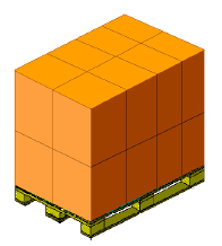
\includegraphics[width=\linewidth]{assets/19.png}
        \caption{UdC Monoarticolo}\label{fig:udc_monoarticolo}
    \end{subfigure}
    \begin{subfigure}{0.33\linewidth}
        \centering
        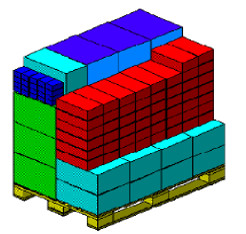
\includegraphics[width=\linewidth]{assets/20.png}
        \caption{UdC Multiarticolo}\label{fig:udc_multiarticolo}
    \end{subfigure}
    \caption{Tipologie di UdC}\label{fig:tipologie_udc}
\end{figure}

%
\section{Carrelli industriali}
I carrelli rappresentano i mezzi di trasporto discontinui più diffusi. Si classificano in base alla capacità di sollevamento (piccolo, medio, grande) e alla modalità di azionamento (manuale o motorizzata).
\subsection{Tipologie di Carrelli}
\begin{enumerate}
    \item \textbf{Transpallet}: Manuali o elettrici, servono per spostamenti orizzontali e piccoli sollevamenti. Richiedono spazi di manovra limitati;
    \item \textbf{Carrelli a forche a sbalzo (Frontali)}: Il classico ``muletto''. Il carico è bilanciato da un contrappeso posteriore. Le caratteristiche tecniche fondamentali includono la portata nominale, l'altezza di sollevamento e il raggio di sterzatura.
    \item \textbf{Carrelli Retrattili}: Il montante o le forche possono ritrarsi, riducendo l'ingombro e permettendo di operare in corridoi più stretti ($ 2.7 $ - $ 3.0 $ m) rispetto ai frontali.
    \item \textbf{Carrelli a Presa Laterale}: Ideali per carichi lunghi e ingombranti. Le versioni moderne sono multidirezionali.
    \item \textbf{Carrelli a Grande Altezza (VNA - Very Narrow Aisle)}: Possono sollevare fino a $ 13 $ - $ 14 $ metri operando in corridoi molto stretti. Possono essere a guida induttiva o con guide di contrasto e avere forche trilaterali.
    \item \textbf{Commissionatori (Order Pickers)}: La cabina si solleva insieme alle forche, permettendo all'operatore di prelevare singoli colli direttamente dallo scaffale.
\end{enumerate}
%
\paragraph{Numero di Carrelli} Per conoscere quanti carrelli sono necessari in un reparto si utilizzano metodi \emph{deterministici} o metodi basati sulla \emph{simulazione al computer}.

Riguardo i metodi deterministici:
\begin{itemize}
    \item Sono veloci, per valutazioni di massima;
    \item L'approccio deterministico è caratterizzato da incertezza;
    \item Sono utili per sistemi con pochi carrelli.
\end{itemize}
\[
    C = \sum_{i}{\frac{N_{i} \cdot t_{i}}{n_{i} \cdot h}}
\]
Dove:
\begin{itemize}
    \item $ C $ è il numero di carrelli;
    \item $ N_{i} $ il numero di unità di carico da trasportare al giorno per ogni articolo $ i $;
    \item $ n_{i} $ il numero di unità di carico dell'articolo $ i $ trasportate da ogni carrello;
    \item $ t_{i} $ tempo richiesto (in ore) dal carrello che trasporta l'articolo $ i $, valutato in base alla velocità del carrello e tenendo conto di curve, incroci, arresti, attività di carico e scarico;
    \item $ h $ il numero di ore lavorative al giorno dei carrelli.
\end{itemize}

%
\subsection{Ingegneria e Sicurezza}
%
\paragraph{Capacità Portante} È definita dal momento ribaltante. La condizione di stabilità è che il momento equilibrante sia maggiore del momento del carico:
\begin{gather*}
    M_{e} = P \cdot e \\
    M_{r} = Q \cdot I \\
    M_{e} > M_{r} \to P \cdot e > Q \cdot I
\end{gather*}
%
\paragraph{Alimentazione} Si sta passando dalle batterie piombo-acido a quelle agli ioni di litio, che permettono ricariche veloci e parziali (biberonaggio), eliminando la necessità di sale ricarica dedicate.

%
\paragraph{Automazione e Sicurezza} L'evoluzione include carrelli a guida autonoma, sistemi anti-collisione e sensori che garantiscono il distanziamento sociale rilevando i tag degli operatori.

%
\section{Trasportatori Meccanici Fissi}
Sistemi di trasporto continuo per flussi elevati e percorsi fissi.
\begin{itemize}
    \item \textbf{A Rulli}: Possono essere folli (a gravità, con pendenza $ 1 $ - $ 6\% $) o motorizzati. Adatti per colli rigidi con fondo regolare. Permettono accumulo e operazioni (imballo, pesatura) lungo il percorso.
    \item \textbf{A Catene}: Utilizzati per carichi pesanti o pallet, costituiti da catene parallele che trascinano il carico.
    \item \textbf{A Nastro}: Per materiali alla rinfusa o carichi leggeri, anche su pendenze. Il nastro può essere piano o concavo.
    \item \textbf{A Piastre (Apron) e Tapparelle}: Costituiti da piastre metalliche o tapparelle trascinate da catene. Molto robusti, usati per carichi pesanti o linee di montaggio.
\end{itemize}

%
\section{Trasportatori per Carichi Elevati}
%
\paragraph{Convogliatore Aerei} Sfruttano lo spazio sopraelevato, liberando il pavimento.
\begin{itemize}
    \item \textbf{Monorotaia}: Una catena a circuito chiuso trascina i carrelli (trolley) su un percorso fisso. Il carico/scarico avviene solitamente in movimento o a bassa velocità;
    \item \textbf{Birotaia (Power \& Free)}: Sistema a due vie. La catena scorre sulla via superiore, mentre i carichi su quella inferiore. Permette di sganciare i carrelli per fermarli (accumulo), cambiare percorso o variare la velocità in sezioni specifiche. È più flessibile ma costoso del monorotaia.
\end{itemize}
%
\paragraph{Carriponte e Gru} Sistemi discontinui per la copertura di aree rettangolari.
\begin{itemize}
    \item \textbf{Carriponte}: Possono essere monotrave (appoggiati o sospesi) o bitrave per portate maggiori. I modelli sospesi riducono gli ostacoli a pavimento eliminando i pilastri di sostegno;
    \item \textbf{Gru a Bandiera}: Utilizzate per servire postazioni di lavoro singole con un raggio d'azione limitato.
\end{itemize}

%
\section{Trasporti Interni e Lean Production}
In ottica Lean, la scelta del mezzo impatta l'efficienza del flusso:
\begin{itemize}
    \item \textbf{Nastri lunghi e Carrelli a forche}: Sono considerati ``negativi'' o da limitare perché creano barriere, incoraggiano grandi lotti e occupano spazio.
    \item \textbf{Trattorini (Tugger trains)}: Una soluzione migliore (``Meglio'') perché seguono rotte regolari (milk-run) e gestiscono contenitori più piccoli.
    \item \textbf{Carrelli manuali}: Considerati ``Il meglio'' per la massima flessibilità, costo nullo di breakdown e promozione del flusso a piccoli lotti, gestiti direttamente dagli addetti.
\end{itemize}
